%   % !TEX root = ../../VIII,3_Rahmen-TeX_8-1.tex
%
%
%   Band VIII, 3 N.~??A19
%   Signatur/Tex-Datei: LH_35_10_17_005-008
%   RK-Nr. 60140 (= L2) + 60141 (= L1)
%   Überschrift: [Appendix de vi absoluta]
%   Datierung: [Janaur bis April 1690]
%   WZ: // RK 60140: LEd8-WZ 803039 = RK-WZ ??? (eins) // RK 60141: LEd8-WZ 803012 = RK-WZ 42e / 409 / 767 (ein Fragment)
%   SZ: (keins)
%   Bilddateien (PDF): LH_35_10_17_005-008_d1; LH_35_10_17_005-008_d2; LH_35_10_17_005-008_d3 (insgemsamt 3)
%
%   NB: Text kollationiert aus L1 (RK 60141) und L2 (RK 60140)
%
%
\selectlanguage{ngerman}%
\frenchspacing%
%
\begin{ledgroupsized}[r]{120mm}
\footnotesize
\pstart
\noindent
\textbf{Überlieferung:}
\pend
\end{ledgroupsized}
%
\begin{ledgroupsized}[r]{114mm}
\footnotesize
\pstart
\parindent -6mm
\makebox[6mm][l]{\textit{L\textsuperscript{1}}}%
Konzept:
LH~XXXV~10,~17 Bl.~7\textendash8. % RK 60141
Ein Bogen~8\textsuperscript{o};
Fragment eines Wasserzeichens auf Bl.~8:
italienisches Papier.
Vier stark bearbeitete Seiten;
Tintenwechsel ab der zweiten Zeile von Bl.~7~v\textsuperscript{o}.
Das Diagramm \lbrack\textit{Fig.~2}\rbrack\ ist in zweifacher Anfertigung (auf Bl.~7~v\textsuperscript{o} und 8~r\textsuperscript{o}) überliefert.
\pend
\end{ledgroupsized}
%
\begin{ledgroupsized}[r]{114mm}
\footnotesize
\pstart
\parindent -6mm
\makebox[6mm][l]{\textit{L\textsuperscript{2}}}%
Reinschrift von \textit{L\textsuperscript{1}} mit Verbesserungen:
LH~XXXV~10,~17 Bl.~5\textendash6 % RK 60140
(unsere Druckvorlage).
Ein Bogen~4\textsuperscript{o};
ein Wasserzeichen mittig:
Papier der Klostermühle zu Thierhaupten.
Drei Seiten;
Bl.~6~v\textsuperscript{o} ist leer.
\pend
\end{ledgroupsized}
%
\selectlanguage{latin}%
\frenchspacing%
%
%
%
\count\Bfootins=1000
\count\Afootins=1200
\count\Cfootins=1000
%
%
%
\vspace{8mm}%    GETRIXT !!!! Sollten 8mm sein !!!!
\pstart%
\normalsize%
\noindent%
%
\lbrack5~r\textsuperscript{o}\rbrack\ % Blatt 5r
%
% MARGINALIE ANFANG
\edtext{}{\lemma{\textit{L\textsuperscript{1},}}\Afootnote{%
\hspace{-1,0mm}\textit{am Rand:}
So kan es abgeschrieben werden als appendix de vi absoluta.\vspace{-4mm}}}%
% MARGINALIE ENDE
\edtext{%
Clarissimus\edlabel{LH_35_10_17_005r+007r_conmech-1}%
\edtext{ quidam Mathematicus\protect\index{Sachverzeichnis}{mathematicus}
in libro\protect\index{Sachverzeichnis}{liber} quem molitur%
\textso{ \textit{de Conatu Mechanico}, }\protect\index{Sachverzeichnis}{conatus mechanicus}}{%
\lemma{Clarissimus \lbrack...\rbrack\ \textso{\textit{Mechanico}}\,}
\Cfootnote{\textsc{G.\,B.\,Boccabadati}, \textit{De conatu mechanico}.\cite{01237}
Die Abhandlung blieb un\-veröffentlicht und gilt als verschollen.}}%
\edlabel{LH_35_10_17_005r+007r_conmech-2}%
optime asserit,
non magis tendi chordam\protect\index{Sachverzeichnis}{chorda tensa}%
}{%
\lemma{\lbrack7~r\textsuperscript{o}\rbrack}\Bfootnote{\hspace{-0,5mm}%
\textbar~Cl.\textsuperscript{mus}\!
\textit{(1)}~B\textlangle occabada\textrangle tus Mutinensium%
\protect\index{Namensregister}{\textso{Boccabadati} (Boccabadatus), Giovan Battista 1635\textendash1696}
\textit{(2)}~quidam Mathematicus \lbrack...\rbrack\ molitur \textit{de Conatu Mechanico} optime asserit \textit{erg.}~%
\textbar\ Non magis
\textit{(1)}~tenditur chorda
\textit{(2)}~tendi chordam%
~\textit{L\textsuperscript{1}}\hspace{0,5mm}
\lbrack5~r\textsuperscript{o}\rbrack\
Clarissimus quidam \lbrack...\rbrack\ tendi chordam%
~\textit{L\textsuperscript{2}}}}
%
a duobus ponderibus
\edtext{aequalibus}{%
\lemma{aequalibus}\Bfootnote{\textit{erg.~L\textsuperscript{1}}}}
%
in diversa trahentibus,\protect\index{Sachverzeichnis}{pondus trahens}
quam ab
\edtext{uno eorum solo}{%
\lemma{uno}\Bfootnote{%
\textit{(1)}~solo
\textit{(2)}~eorum solo%
~\textit{L\textsuperscript{1}}}}
% \hspace{0,5mm}
% eorum solo%
% ~\textit{L\textsuperscript{2}}
%
eandem
\edtext{chordam}{%
\lemma{chordam}\Bfootnote{\textit{fehlt~L\textsuperscript{1}}}}
%
muro\protect\index{Sachverzeichnis}{murus}
affixam\protect\index{Sachverzeichnis}{chorda affixa}
\edtext{trahente.\protect\index{Sachverzeichnis}{pondus trahens} Et}{%
\lemma{trahente.}\Bfootnote{%
\hspace{-0,5mm}%
\textbar~Quod facile demonstratu, intelligendo enim alterutrum
\textit{(1)}~eorum
\textit{(2)}~ponderum muro aggelascere, non ideo mutatur tensio.
\textit{gestr.}~\textbar\ Et%
~\textit{L\textsuperscript{1}}}}
%
sane
%
\edtext{(\protect\vphantom)%
mea sententia\protect\index{Sachverzeichnis}{sententia}%
\protect\vphantom()}{%
\lemma{mea}\Bfootnote{%
\hspace{-0,5mm}sententia
\textit{erg.~L\textsuperscript{1}}
\hspace{0,5mm}%
(\protect\vphantom)mea sententia\protect\vphantom()%
~\textit{L\textsuperscript{2}}}}
%
pondus
%
\edtext{oppositum\protect\index{Sachverzeichnis}{pondus oppositum}
vicem muri\protect\index{Sachverzeichnis}{murus} subit;}{%
\lemma{oppositum}\Bfootnote{\hspace{-0,5mm}%
\textit{(1)}~muro
\textit{(2)}~muri vicem subit,%
~\textit{L\textsuperscript{1}}
\hspace{0,5mm}oppositum
\textit{(1)}~muri
\textit{(2)}~vicem muri subit;%
~\textit{L\textsuperscript{2}}}}
%
sufficit enim tantam 
\edtext{id}{%
\lemma{id}\Bfootnote{%
\textit{erg.~L\textsuperscript{1} u.~L\textsuperscript{2}}}}
%
vim\protect\index{Sachverzeichnis}{vis ponderis} habere,
ut a pondere\protect\index{Sachverzeichnis}{pondus trahens} 
%
\edtext{priore \lbrack chorda\rbrack\ non trahi patiatur,}{%\protect\index{Sachverzeichnis}{chorda tracta}
\lemma{priore}\Bfootnote{%
\hspace{-0,5mm}chordam non trahi
\textit{(1)}~ponatur;
\textit{(2)}~patiatur;%
~\textit{L\textsuperscript{1}}
\hspace{0,5mm}priore
\textbar~chordam \textit{ändert Hrsg.}~%
\textbar\ non trahi patiatur,%
~\textit{L\textsuperscript{2}}}}
%
seu ut chorda integra\protect\index{Sachverzeichnis}{chorda integra} moveri non possit%
\edtext{, alioqui tensio\protect\index{Sachverzeichnis}{tensio chordae} eluderetur.}{%
\lemma{\hspace{-1,0mm}, alioqui}\Bfootnote{%
\hspace{-0,5mm}tensio eluderetur\,
\textit{fehlt~L\textsuperscript{1},
erg.~L\textsuperscript{2}}}}
%
Et ex
%
\edtext{pondere illo retinente,\protect\index{Sachverzeichnis}{pondus retinens}
murum\protect\index{Sachverzeichnis}{murus} facere,}{%
\lemma{pondere}\Bfootnote{%
\hspace{-0,5mm}%
\textbar~illo retinente \textit{erg.}%
~\textbar\ murum facere%
~\textit{L\textsuperscript{1}}
\hspace{0,5mm}pondere illo retinente, murum facere,%
~\textit{L\textsuperscript{2}}}}
%
nihil aliud est
\edtext{quam in ipso potentiam}{%
\lemma{quam}\Bfootnote{%
\textit{(1)}~pondus
\textit{(2)}~ejus
\textit{(3)}~in ipso potentiam%
~\textit{L\textsuperscript{1}}}}
% \hspace{0,5mm}
% in ipso potentiam%
% ~\textit{L\textsuperscript{2}}
%
resistendi\protect\index{Sachverzeichnis}{potentia resistendi} augere,
non aucta
%
\edtext{ipsius}{%
\lemma{ipsius}\Bfootnote{%
\textit{fehlt~L\textsuperscript{1},
erg.~L\textsuperscript{2}}}}
%
potentia\protect\index{Sachverzeichnis}{potentia trahendi}
%
\edtext{trahendi.
Quod}{%
\lemma{trahendi~,}\Bfootnote{%
\hspace{-0,5mm}quod%
~\textit{L\textsuperscript{1}}
\hspace{0,5mm}trahendi~. Quod%
~\textit{L\textsuperscript{2}}}}
%
\makebox[1.0\textwidth][s]{idem est
ac si pondus fieret immensum,\protect\index{Sachverzeichnis}{pondus immensum}
sed ei supponeretur
%
\edtext{sufficiens}{%
\lemma{sufficiens}\Bfootnote{\hspace{-0,5mm}%
\textit{erg.~L\textsuperscript{1}}}}
%
\edtext{sustentaculum,\protect\index{Sachverzeichnis}{sustentaculum}}{%
\lemma{sustentaculum~;~\textit{L\textsuperscript{1}}}\Bfootnote{%
\hspace{0,5mm}sustentaculum~,%
~\textit{L\textsuperscript{2}}}}
%
ut}
\pend
\count\Bfootins=900
\count\Afootins=1000
\count\Cfootins=900
\newpage
%
  \centerline{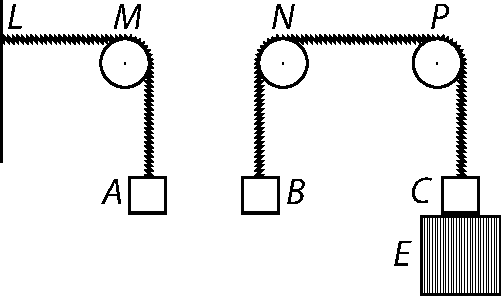
\includegraphics[width=0.38\textwidth]{gesamttex/edit_VIII,3/images/LH_35_10_17_005-008_d1.pdf}}%
  \vspace{0.5em}
  \centerline{\lbrack\textit{Fig.~1; L\textsuperscript{1}\! (Bl.~7~r\textsuperscript{o}\!) u. L\textsuperscript{2}\! (Bl.~5~r\textsuperscript{o}\!)}\rbrack}%
%
 \vspace{1.5em}%
\pstart\noindent
\edtext{infinite quidem}{%
\lemma{infinite}\Bfootnote{%
\hspace{-0,5mm}quidem
\textit{erg.~L\textsuperscript{1}}}}
%
resistere possit
%
\edtext{elevanti,\protect\index{Sachverzeichnis}{pondus elevans}
seu chordam\protect\index{Sachverzeichnis}{chorda tracta}
trahenti,\protect\index{Sachverzeichnis}{pondus trahens}
sed}{%
\lemma{elevanti,}\Bfootnote{%
\hspace{-0,5mm}\textbar~seu chordam trahenti. Sed
\textit{erg.}~\textbar%
~\textit{L\textsuperscript{1}}
\hspace{0,5mm}elevanti, seu chordam trahenti, sed%
~\textit{L\textsuperscript{2}}}}
%
descendere
\edtext{non possit.
Ita quantacunque}{%
\lemma{non}\Bfootnote{%
\hspace{-0,5mm}possit
\textit{(1)}~quantacunque autem
\textit{(2)}~.~Ita quantacunque%
~\textit{L\textsuperscript{1}}}}
% \hspace{0,5mm}
% .~Ita quantacunque%
% ~\textit{L\textsuperscript{2}}
%
\edtext{ponderis\protect\index{Sachverzeichnis}{pondus retinens}
\lbrack retinentis\rbrack\
magnitudo sit,\protect\index{Sachverzeichnis}{magnitudo ponderis}
superfluum}{%
\lemma{ponderis}\Bfootnote{%
\textit{(1)}~pote
\textit{(2)}~retinentis
\textit{(a)}~,~vel resi
\textit{(b)}~magnitudo sit,
\textbar~vel quantacunque sit resistentia contra chordae integrae tractionem \textit{gestr.}~%
\textbar\ superfluum%
~\textit{L\textsuperscript{1}}
\hspace{0,5mm}ponderis
\textbar~renitentis \textit{ändert Hrsg. nach~L\textsuperscript{1}}~%
\textbar\ magnitudo sit, superfluum%
~\textit{L\textsuperscript{2}}}}
%
est, quicquid trahentis vim\protect\index{Sachverzeichnis}{pondus trahens}\protect\index{Sachverzeichnis}{vis ponderis}
\edtext{excedit.
Tenduntur autem ipsae fibrae\protect\index{Sachverzeichnis}{fibra} muri\protect\index{Sachverzeichnis}{murus}
vel obstaculi resistentis,\protect\index{Sachverzeichnis}{obstaculum resistens}}{%
\lemma{excedit.}\Bfootnote{%
\textit{(1)}~Tenditur autem ipse murus resiste
\textit{(2)}~Tenduntur autem
\textbar~ipsae \textit{erg.}~%
\textbar\ fibrae
\textit{(a)}~seu
\textit{(b)}~muri vel obstaculi
\textit{(aa)}~\textlangle praemo\textrangle ti
\textit{(bb)}~resistentis,%
~\textit{L\textsuperscript{1}}}}
% \hspace{0,5mm}
% Tenduntur autem \lbrack...\rbrack\ obstaculi resistentis,%
% ~\textit{L\textsuperscript{2}}
%
pro vi ponderis\protect\index{Sachverzeichnis}{vis ponderis}
oppositi\protect\index{Sachverzeichnis}{pondus oppositum}
trahentis,\protect\index{Sachverzeichnis}{pondus trahens}
idque perinde
%
\edtext{est}{%
\lemma{est~,~\textit{L\textsuperscript{1}}}\Bfootnote{%
\hspace{0,5mm}est~\textit{L\textsuperscript{2}}}}
%
ac si chorda\protect\index{Sachverzeichnis}{chorda tracta} in tantundem esset
\edlabel{LH_35_10_17_005r_veriss-1}%
continuata.
\edtext{}{%
{\xxref{LH_35_10_17_005r_veriss-1}{LH_35_10_17_005r_veriss-2}}%
{\lemma{continuata.}\Bfootnote{%
\textit{(1)}~Ex Epistola mea ad Cl. Boccabadatum 
\textit{(2)}~Sed haec distinctius explicare pretium operae est, \lbrack...\rbrack\ error oboriatur. % quis inde
\textit{(a)}~Assen
\textit{(b)}~Verissimum est
\textit{(c)}~Quanquam verum sit tantundem chordam unius
\textit{(d)}~Verissimum \textbar~quidem \textit{erg.}~\textbar\ est chordam \textit{LM} muro \textit{L}
\textit{(aa)}~infixam
\textit{(bb)}~affixam tantundem tendi a pondere \textit{A} unius%
~\textit{L\textsuperscript{1}}
\hspace{0,5mm}continuata. Sed \lbrack...\rbrack\ pondere \textit{A}, unius%
~\textit{L\textsuperscript{2}}}}}%
\edtext{%
\edlabel{LH_35_10_17_005r_variant-1}%
Sed haec distinctius explicare operae pretium est,
ne quis inde error\protect\index{Sachverzeichnis}{error} oboriatur.%
\edlabel{LH_35_10_17_005r_variant-2}%
}{%
\lemma{continuata. \lbrack...\rbrack\ oboriatur}\Cfootnote{%
Der in der Variante \textit{(1)} von \textit{L\textsuperscript{1}} erwähnte Brief an Boccabadati ist nicht bekannt.
In einem Brief an B.~Ramazzini vom 25. Februar 1690 verweist Leibniz aber auf den Austausch mit Boccabadati über verwandte Themen:
\textit{In literis ad Dn. Boccabadatum quaedam attigi de Motus Tonici aestimatione}
(\cite{01238}\textit{LSB} III,~4 N.~239, S.~467.11\textendash12).}}%
% % % % %    ACHTUNG GETRIXT: FOLGENDE CFOOTNOTE HÄNGT AN FIG. 1    ! ! ! ! 
% \edtext{}{\lemma{\hspace{1,6mm}\lbrack\textit{Fig.~1}\rbrack}\killnumber\Cfootnote{%
% In \textit{L\textsuperscript{1}} auf Bl.~7~r\textsuperscript{o}.}}
\pend%
%
%
%  \newpage
 \pstart%
Verissimum quidem est chordam \textit{LM},
muro \textit{L}\protect\index{Sachverzeichnis}{murus}
affixam\protect\index{Sachverzeichnis}{chorda affixa}
tantundem tendi a pondere \textit{A},\protect\index{Sachverzeichnis}{pondus tendens}
unius%
\edlabel{LH_35_10_17_005r_veriss-2}
(\vphantom)si
placet\vphantom()
%
\edtext{librae,\protect\index{Sachverzeichnis}{libra}}{%
\lemma{librae~;~\textit{L\textsuperscript{1}}}\Bfootnote{%
\hspace{0,5mm}librae~,~\textit{L\textsuperscript{2}}}}
%
quantum chorda\protect\index{Sachverzeichnis}{chorda tensa}
\edtext{similis priori, \textit{NP}}{%
\lemma{similis}\Bfootnote{%
\hspace{-0,5mm}\textbar~priori \textit{erg.}~\textbar\
\textit{NP},%
~\textit{L\textsuperscript{1}}
\hspace{0,5mm}similis priori, \textit{NP}%
~\textit{L\textsuperscript{2}}}}
%
\edtext{tenditur a}{%
\lemma{tenditur}\Bfootnote{% 
\hspace{-0,5mm}a \textit{erg.~L\textsuperscript{1}}}}
%
duobus ponderibus\protect\index{Sachverzeichnis}{pondus tendens}
\textit{B} et \textit{C},
quorum quodlibet etiam est
%
\edtext{unius librae\protect\index{Sachverzeichnis}{libra}
\edtext{\lbrack idque}{%
\lemma{\lbrack idque\,}\Cfootnote{%
Eckige Klammer von Leibniz.}}%
}{\lemma{unius}\Bfootnote{% 
\hspace{-0,5mm}librae, idque%
~\textit{L\textsuperscript{1}}
\hspace{0,5mm}unius
\textit{(1)}~librae, idque
\textit{(2)}~librae \lbrack idque%
~\textit{L\textsuperscript{2}}}}
%
sic facile demonstratur:
ponamus pondus \textit{C}
%
\edtext{aggelascere\protect\index{Sachverzeichnis}{pondus aggelatum}
scabello\protect\index{Sachverzeichnis}{scabellum} supposito, \textit{E};
utique inde non mutatur tensio.\protect\index{Sachverzeichnis}{tensio chordae}
Jam perinde tunc erit,
ac si}{%
\lemma{aggelascere}\Bfootnote{\hspace{-0,5mm}%
\textit{(1)}~suppedaneo c
\textit{(2)}~scabello supposito \textit{E,}
\textit{(a)}~utique perinde est ac si
\textit{(b)}~utique inde \lbrack...\rbrack\ tunc erit ac si%
~\textit{L\textsuperscript{1}}
\hspace{0,5mm}aggelascere scabello \lbrack...\rbrack\ ac si%
~\textit{L\textsuperscript{2}}}}
%
\edtext{chorda \textit{BNPC}}{%
\lemma{chorda}\Bfootnote{%
\textit{(1)}~\textit{NPC}
\textit{(2)}~\textit{BNPC}%
~\textit{L\textsuperscript{1}}}}
% \hspace{0,5mm}
% \textit{BNPC}%
% ~\textit{L\textsuperscript{2}}
%
\edtext{esset uno extremo \textit{C}
affixa\protect\index{Sachverzeichnis}{chorda affixa}
muro\protect\index{Sachverzeichnis}{murus} \textit{E}.}{%
\lemma{esset}\Bfootnote{\hspace{-0,5mm}%
\textit{(1)}~muro
\textit{(2)}~uno extremo \textit{C}
\textit{(a)}~infixa
\textit{(b)}~affixa muro \textit{E}.%
~\textit{L\textsuperscript{1}}
% \hspace{0,5mm}esset uno \lbrack...\rbrack\ muro \textit{E}.%
% ~\textit{L\textsuperscript{2}}
}}
%
Unus ergo
\edtext{casus
(\protect\vphantom)%
duorum ponderum%
\protect\vphantom()
ad alterum
(\protect\vphantom)%
unius ponderis et muri\protect\index{Sachverzeichnis}{murus}%
\protect\vphantom()}{%
\lemma{casus}\Bfootnote{%
\textit{(1)}~ad alterum
\textit{(2)}~(\protect\vphantom)duorum ponderum\protect\vphantom() \lbrack...\rbrack\ et muri\protect\vphantom()%
~\textit{L\textsuperscript{1}}}}
% \hspace{0,5mm}
% (\protect\vphantom)duorum ponderum\protect\vphantom() \lbrack...\rbrack\ et muri\protect\vphantom()%
% ~\textit{L\textsuperscript{2}}
%
tanquam aequivalentem\protect\index{Sachverzeichnis}{casus aequivalens}
%
\edtext{reducitur.\rbrack}{%
{\lemma{reducitur.\rbrack\,}\Cfootnote{%
Eckige Klammer von Leibniz.\hspace{1.7mm}}}%
{\lemma{reducitur.~\textit{L\textsuperscript{1}}}\Bfootnote{%
\hspace{0,5mm}reducitur.~\rbrack~\textit{L\textsuperscript{2}}}}}
%
Sed\edlabel{LH_35_10_17_005-008_tensioindet-1} hinc
\edtext{non sequitur
(\protect\vphantom)%
meo judicio\protect\index{Sachverzeichnis}{iudicium}%
\protect\vphantom()}{%
\lemma{non}\Bfootnote{%
\textit{(1)}~puto
\textit{(2)}~sequitur (\protect\vphantom)meo judicio\protect\vphantom()%
~\textit{L\textsuperscript{1}}}}
% \hspace{0,5mm}
% sequitur (\protect\vphantom)meo judicio\protect\vphantom()%
% ~\textit{L\textsuperscript{2}}
%
\edtext{vim quam}{%
\lemma{vim}\Bfootnote{%
\hspace{-0,5mm}\lbrack7~v\textsuperscript{o}\rbrack\ quam%
~\textit{L\textsuperscript{1}}}}
%
patitur\protect\index{Sachverzeichnis}{vis tendens}
%
\edtext{chorda\protect\index{Sachverzeichnis}{chorda tensa} \textit{LMA}, vel \mbox{\textit{BNPC}}}{%
\lemma{chorda}\Bfootnote{\hspace{-0,5mm}%
\textit{(1)}~\textit{LM}
\textit{(2)}~\textit{LMA} \textbar~vel \textit{BNPC} \textit{erg.}~\textbar%
~\textit{L\textsuperscript{1}}
\hspace{0,5mm}chorda
\textit{LMA}, vel \textit{BNPC}%
~\textit{L\textsuperscript{2}}}}
%
esse duplam potentiae\protect\index{Sachverzeichnis}{potentia ponderis}
%
\edtext{ponderis \textit{A},
seu esse aequalem simul potentiae ponderum\protect\index{Sachverzeichnis}{potentia ponderis}
\textit{B} et \textit{C}.}{%
\lemma{ponderis}\Bfootnote{\hspace{-0,5mm}%
\textit{(1)}~\textit{A}
\textit{(2)}~\textit{A}
\textbar~seu esse \lbrack...\rbrack\ \textit{B} et \textit{C} \textit{erg.}~%
\textbar~.~\textit{L\textsuperscript{1}}
\hspace{0,5mm}ponderis
\textit{A} \lbrack...\rbrack\ et \textit{C}.%
~\textit{L\textsuperscript{2}}}}%
\edlabel{LH_35_10_17_005-008_tensioindet-2}
%
Sed potius esse
%
\edtext{aequalem uni soli ponderi\protect\index{Sachverzeichnis}{pondus tendens}
ut \textit{B},}{%
\lemma{aequalem}\Bfootnote{%
\hspace{-0,5mm}%
\textbar~uni soli ponderi ut
\textit{(1)}~\textit{A} aut
\textit{(2)}~\textit{B}
\textit{erg.}~\textbar%
~\textit{L\textsuperscript{1}}
\hspace{0,5mm}aequalem uni \lbrack...\rbrack\ ut \textit{B},% soli ponderi
~\textit{L\textsuperscript{2}}}}
%
cum alterutrum
%
\edtext{ponderum\protect\index{Sachverzeichnis}{pondus tendens}
ut \textit{C},
considerari possit tanquam muri\protect\index{Sachverzeichnis}{murus} vicem subiens,
ut non aliud praestet,
quam impedire motum totius chordae,\protect\index{Sachverzeichnis}{motus chordae}
quod ad tensionem\protect\index{Sachverzeichnis}{tensio} necesse est.
Quod si officia\protect\index{Sachverzeichnis}{officium}
inter duo pondera\protect\index{Sachverzeichnis}{pondus tendens}
\textit{B} et \textit{C} partiri volumus,
utrumquodque pro parte muri\protect\index{Sachverzeichnis}{murus} resistentis,
pro parte potentiae tendentis\protect\index{Sachverzeichnis}{potentia tendens}
officium\protect\index{Sachverzeichnis}{officium} faciet.
Quod ut appareat}{%
\lemma{ponderum~,}\Bfootnote{\hspace{-0,5mm}%
\textit{(1)}~muri locum habeat, nec locum habeat tensio nisi
\textit{(a)}~\textlangle motus chor\textrangle % 
\textit{(b)}~sit quod prohibeat motionem totius chordae
\textit{(2)}~\textbar~ut \textit{C} considerari possit tanquam \textit{erg.}~\textbar\ muri vicem
\textit{(a)}~subiret nec aliud praestaret
\textit{(b)}~subiens ut non aliud praestet quam
\textit{(aa)}~ut impediat
\textit{(bb)}~impedire motum totius chordae quod ad tensionem necesse est.
\textit{(aaa)}~Quod ut appareat
\textit{(bbb)}~Quod si officia
\textit{(aaaa)}~volumus
\textit{(bbbb)}~inter duo \lbrack...\rbrack\  officium faciet.
\textit{(aaaaa)}~Quatenus autem
\textit{(bbbbb)}~Quod ut appareat%
~\textit{L\textsuperscript{1}}
\hspace{0,5mm}ponderum ut \textit{C}, \lbrack...\rbrack\ Quod ut appareat%
~\textit{L\textsuperscript{2}}}}
%
clarius,
%
\lbrack5~v\textsuperscript{o}\rbrack\ % Blatt 5v.
%
ostendam\protect\index{Sachverzeichnis}{casus}
%
\edtext{casum,}{%
\lemma{casum~\textit{L\textsuperscript{1}}}\Bfootnote{%
\hspace{0,5mm}casum~,%
~\textit{L\textsuperscript{2}}}}
%
quo plura
\edtext{\lbrack duobus\rbrack}{%
\lemma{duobus}\Bfootnote{%
\textit{erg.~L\textsuperscript{1},
fehlt~L\textsuperscript{2},
erg. Hrsg. nach~L\textsuperscript{1}}}}
%
pondera aequalia simul
\edtext{eodem modo}{%
\lemma{eodem}\Bfootnote{%
\hspace{-0,5mm}modo
\textit{erg.~L\textsuperscript{1}}}}
%
eidem
%
\edtext{tendibili\protect\index{Sachverzeichnis}{tendibile}}{%
\lemma{Tendibili~\textit{L\textsuperscript{1}}}\Bfootnote{%
%
\hspace{0,5mm}tendibili%
~\textit{L\textsuperscript{2}}}}
%
\edtext{immediate}{%
\lemma{immediate}\Bfootnote{%
\textit{erg.~L\textsuperscript{1}}}}
%
appenduntur,\protect\index{Sachverzeichnis}{pondus appensum}
unde sequeretur tunc tensionem non tantum duplam,
sed
%
\edtext{triplam quadruplamve aut magis adhuc
pro arbitrio\protect\index{Sachverzeichnis}{arbitrium}
multiplam\protect\index{Sachverzeichnis}{tensio multipla} esse
ejus potentiae}{%
\lemma{triplam~,}\Bfootnote{% 
\hspace{-0,5mm}quadruplamve esse,
\textit{(1)}~imo non esse dete
\textit{(2)}~aut magis adhuc multiplam
\textbar~(pro arbitrio) \textit{erg.}~%
\textbar\ potentiae%
~\textit{L\textsuperscript{1}}
\hspace{0,5mm}triplam quadruplamve
\textit{(1)}~esse aut magis adhuc multiplam (pro arbitrio)
\textit{(2)}~aut magis \lbrack...\rbrack\ ejus potentiae%
~\textit{L\textsuperscript{2}}}}
%
%\edtext{}{%
%\lemma{}\Bfootnote{%
%\textit{fehlt~L\textsuperscript{1},
%erg.~L\textsuperscript{2}}}}
%
quam unum pondus
\edtext{exercet,\protect\index{Sachverzeichnis}{potentia ponderis}
adeoque nullius}{%
\lemma{exercet,}\Bfootnote{%
\textit{(1)}~imo
\textit{(2)}~nullam
\textit{(3)}~null
\textit{(4)}~\textbar~adeoque \textit{erg.}~\textbar\ nullius%
~\textit{L\textsuperscript{1}}}}
%
esse
\edtext{ad eam}{%
\lemma{ad}\Bfootnote{%
\hspace{-0,5mm}eam
\textit{erg.~L\textsuperscript{1}}}}
%
proportionis\protect\index{Sachverzeichnis}{proportio determinata}
%
\edtext{determinatae,}{%
\lemma{determinatae~\textit{L\textsuperscript{1}}}\Bfootnote{%
\hspace{0,5mm}determinatae~,%
~\textit{L\textsuperscript{2}}}}
%
quod absurdum\protect\index{Sachverzeichnis}{absurdum} foret.
%
\edtext{Nam qua ratione proportio dupla tensionis chordae\protect\index{Sachverzeichnis}{tensio chordae}
ad unum ex ponderibus\protect\index{Sachverzeichnis}{pondus tendens} concludi posset,
eo argumento\protect\index{Sachverzeichnis}{argumentum} et alia quaevis concludi potest,
cum multiplicatis ponderibus\protect\index{Sachverzeichnis}{pondus multiplicatum}
tensio\protect\index{Sachverzeichnis}{tensio chordae} non augeatur,
\edtext{ut jam patebit.}{\lemma{ut jam patebit}\Cfootnote{%
\hspace{1mm}Vgl.\hspace{0.2mm} S.~\refpassage{LH_35_10_17_005-008_tensioindet-3}{LH_35_10_17_005-008_tensioindet-4}.}}}{%
\lemma{Nam}\Bfootnote{%
\hspace{-0,5mm}qua \lbrack...\rbrack\ quaevis concludi potest,
\textso{cum multiplicatis ponderibus} tensio \lbrack...\rbrack\ jam patebit.
\textit{erg.~L\textsuperscript{1}}
\hspace{0,5mm}Nam qua \lbrack...\rbrack\ ponderibus concludi
\textit{(1)}~potest,
\textit{(2)}~posset, eo argumento \lbrack...\rbrack\ jam patebit.%
~\textit{L\textsuperscript{2}}}}
\pend%
%
%
\pstart%
Casus\protect\index{Sachverzeichnis}{casus}
autem plurium duobus ponderum simul
%
\edtext{appensorum\protect\index{Sachverzeichnis}{pondus appensum}
obtineri potest ope fluidi}{%
\lemma{appensorum}\Bfootnote{%
\textit{(1)}~obtinebit
\textit{(2)}~obtineri potest ope
\textit{(a)}~liquidi
\textit{(b)}~fluidi%
~\textit{L\textsuperscript{1}}}}
%
tendibilis,\protect\index{Sachverzeichnis}{fluidum tendibile}
quod etsi fortasse non detur apud nos,
fingi tamen potest.
%
\edtext{Et talem esse aerem\protect\index{Sachverzeichnis}{aer} sibi fingunt,
qui ejus \edtext{pressionem\protect\index{Sachverzeichnis}{pressio aeris}
et Elastrum\protect\index{Sachverzeichnis}{elastrum aeris} non}{%
{\lemma{pressionem}\Bfootnote{\hspace{-0,5mm}%
\textit{(1)}~in
\textit{(2)}~et elastrum
\textbar~a Torricellio\protect\index{Namensregister}{\textso{Torricelli} (Torricellius), Evangelista 1608\textendash1647} inventum \textit{gestr.}~%
\textbar\ non%
~\textit{L\textsuperscript{1}}
\hspace{0,5mm}pressionem et Elastrum non%
~\textit{L\textsuperscript{2}}}}%
{\lemma{pressionem et Elastrum}\Cfootnote{%
Im gestr. Text der Variante \textit{(2)} von \textit{L\textsuperscript{1}} Anspielung auf den experimentellen Nachweis des Luftdrucks,
von dem E.~Torricelli in seinem Brief an Ricci vom 11. Juni 1644 berichtet hatte.%
\protect\index{Namensregister}{\textso{Torricelli} (Torricellius), Evangelista 1608\textendash1647}
Vgl. C.~\textsc{Dati}, \textit{Lettera a Filaleti ... della famosissima esperienza dell'argento vivo}, Florenz 1663, S.~20\,f.;\cite{00107} E.~\textsc{Torricelli}, \textit{Opere}, Bd.~III, Faenza 1919, S.~186\textendash188.\cite{00108}}}}
%
admittentes,
putant Mercurium\protect\index{Sachverzeichnis}{mercurium}
in Tubo Torricelliano\protect\index{Sachverzeichnis}{tubus Torricellianus}
suspendi ab aere
incluso\protect\index{Sachverzeichnis}{aer inclusus}
rarefacto,\protect\index{Sachverzeichnis}{aer rarefactus}
velut a
%
\edtext{funiculo.\protect\index{Sachverzeichnis}{funiculus}
Quod}{%
\lemma{funiculo~;}\Bfootnote{%
\hspace{-0,5mm}quod%
~\textit{L\textsuperscript{1}}
\hspace{0,5mm}funiculo~. Quod%
~\textit{L\textsuperscript{2}}}}%
}{%
\lemma{Et talem \lbrack...\rbrack\  funiculo}\Cfootnote{%
Anspielung auf die von der \glqq Funiculus-Hypothese\grqq\ herrührende Erklärung pneumatischer Phänomene in F.~\textsc{Linus}, \textit{Tractatus de corporum inseparabilitate}, London 1661.\cite{00072}}}
%
quamvis falsum sit,
servit tandem haec fictio\protect\index{Sachverzeichnis}{fictio} non impossibilis
declarandae ratiocinationi\protect\index{Sachverzeichnis}{ratiocinatio} meae.
%
%
\edtext{Fingamus}{%
\lemma{Fingamus}\Cfootnote{%
Siehe \lbrack\textit{Fig.~2}\rbrack\ auf S.~\pageref{LH_35_10_17_008r_Fig2}.}}
%
ergo
%
\edtext{vas\protect\index{Sachverzeichnis}{vas fluido tendibili plenum} \textit{A},
firmum ut loco moveri nequeat,
fluido tendibili\protect\index{Sachverzeichnis}{fluidum tendibile} plenum,
accurate clausum nisi quod habet}{%
\lemma{vas}\Bfootnote{%
\hspace{-0,5mm}\textit{A},
\textbar~firmum ut loco moveri nequeat, \textit{erg.}~\textbar\
accurate clausum, fluido tendibili plenum, habens%
~\textit{L\textsuperscript{1}}
\hspace{0,5mm}vas \textit{A},
\textit{(1)}~accurate clausum, fluido tendibili plenum, habens
\textit{(2)}~firmum ut \lbrack...\rbrack\ quod habet%
~\textit{L\textsuperscript{2}}}}
%
tres vel plures exitus\protect\index{Sachverzeichnis}{exitus tubiformis}
%
\edtext{tubiformes aequales \textit{1.2}; et \textit{3.4}; et \textit{5.6}, etc.
quos accurate impleant
emboli\protect\index{Sachverzeichnis}{embolus}
\textit{7.8}; \textit{9.10}; \textit{11.12}; etc.
nempe tam tubis quam embolis ita perfecte tornatis,%
\protect\index{Sachverzeichnis}{embolus tornatus}\protect\index{Sachverzeichnis}{tubus tornatus}
ut emboli sine ullo obstaculo\protect\index{Sachverzeichnis}{obstaculum} intra tubos
salva obturatione\protect\index{Sachverzeichnis}{obturatio} moveantur.
Hi emboli trahantur\protect\index{Sachverzeichnis}{embolus tractus}
a ponderibus\protect\index{Sachverzeichnis}{pondus trahens}}{%
\lemma{tubiformes~,}\Bfootnote{%
\textit{(1)}~quo
\textit{(2)}~aequales \textit{1.2}, \textit{3.4}, \textit{5.6}
\textbar~etc. \textit{erg.}~\textbar~; quos
\textit{(a)}~exacte clau
\textit{(b)}~accurate
\textit{(aa)}~implent
\textit{(bb)}~impleant emboli \textit{7.8}, \textit{9.10}, \textit{11.12} etc.
\textit{(aaa)}~qui emboli trahantur a po
\textit{(bbb)}~et ita perfecte
\textit{(aaaa)}~respondent,
\textit{(bbbb)}~respondeant, ut
\textit{(ccc)}~% \textbar~nempe \textit{fehlt}~\textbar\ 
tam tubis \lbrack...\rbrack\ % quam embolis ita 
perfecte tornatis, ut emboli \lbrack...\rbrack\ intra tubos % sine ullo obstaculo 
\textbar~salva obturatione \textit{erg.}~%
\textbar\ moveantur. Hi \lbrack...\rbrack\ a ponderibus% emboli trahantur 
~\textit{L\textsuperscript{1}}
\hspace{0,5mm}tubiformes aequales \lbrack...\rbrack\ perfecte tornatis,
\textbar~ita \textit{streicht Hrsg. nach~L\textsuperscript{1}}~\textbar\
ut emboli \lbrack...\rbrack\ a ponderibus%
~\textit{L\textsuperscript{2}}}}
%
\textit{B}, \textit{C}, \textit{D} inter se aequalibus,
donec fluidum tendibile\protect\index{Sachverzeichnis}{fluidum tendibile}
vasi\protect\index{Sachverzeichnis}{vas} \textit{A}
%
\edtext{inclusum}{%
\lemma{inclusum~,~\textit{L\textsuperscript{1}}}\Bfootnote{%
\hspace{0,5mm}inclusum~\textit{L\textsuperscript{2}}}}
%
ad certum tensionis\protect\index{Sachverzeichnis}{tensio}
\edtext{\lbrack vel dilatationis\rbrack}{%
\lemma{vel}\Bfootnote{%
dilatationis\protect\index{Sachverzeichnis}{dilatatio}
\textit{erg.~L\textsuperscript{1},
fehlt~L\textsuperscript{2},
erg. Hrsg. nach~L\textsuperscript{1}}}}
gradum\protect\index{Sachverzeichnis}{gradus tensionis}\protect\index{Sachverzeichnis}{gradus dilatationis}
perveniat,
%
quem pondera\protect\index{Sachverzeichnis}{pondus appensum} vincere
\edtext{vel augere}{%
\lemma{vel}\Bfootnote{%
\hspace{-0,5mm}augere
\textit{erg.~L\textsuperscript{1}}}}
%
non
\edtext{possint}{%
\lemma{possint~;~\textit{L\textsuperscript{1}}}\Bfootnote{%
\hspace{0,5mm}possint%
~\textit{L\textsuperscript{2}}}}
%
atque ita suspensa
\edtext{maneant,}{
\lemma{\hspace{-0,5mm}maneant~\textit{L\textsuperscript{1}}}\Bfootnote{%
\hspace{0,5mm}maneant~,%
~\textit{L\textsuperscript{2}}}}
%
\edtext{et tam inter se,
quam cum fluidi\protect\index{Sachverzeichnis}{fluidum tendibile}%
\textso{ vi tonica }\protect\index{Sachverzeichnis}{vis tonica}%
aequilibrentur.}{%
\lemma{et}\Bfootnote{%
\hspace{-0,5mm}\textit{(1)}~in aequilibrio\protect\index{Sachverzeichnis}{aequilibrium}
\textit{(2)}~tam inter \lbrack...\rbrack\ fluidi Vi tonica % inter se, quam cum
\textbar~aequilibrentur \textit{erg.}~\textbar~.%
~\textit{L\textsuperscript{1}}
\hspace{0,5mm}et tam \lbrack...\rbrack\ \textso{tonica} aequilibrentur.%
~\textit{L\textsuperscript{2}}}}
%
Jam
\edtext{fingamus}{%
\lemma{fingamus~;~\textit{L\textsuperscript{1}}}\Bfootnote{%
\hspace{0,5mm}fingamus%
~\textit{L\textsuperscript{2}}}}
%
\edtext{omnia \lbrack haec\rbrack\ pondera}{%
\lemma{omnia}\Bfootnote{\hspace{-0,5mm}%
haec \lbrack8~r\textsuperscript{o}\rbrack\ pondera,%
~\textit{L\textsuperscript{1}}
\hspace{0,5mm}omnia
\textbar~haec \textit{erg. Hrsg. nach~L\textsuperscript{1}}~%
\textbar\ pondera%
~\textit{L\textsuperscript{2}}}}
%
(\protect\vphantom)%
ut \textit{C}, \textit{D}
\edtext{etc.}{%
\lemma{etc.}\Bfootnote{%
\textit{erg.~L\textsuperscript{1}}}}%
\protect\vphantom()
%
dem\-to uno \textit{B},
aggelascere\protect\index{Sachverzeichnis}{pondus aggelatum}
suppedaneis\protect\index{Sachverzeichnis}{suppedaneum}
seu
\edtext{sustentaculis\protect\index{Sachverzeichnis}{sustentaculum}
(\protect\vphantom)%
\textit{E}, \textit{F}, etc.%
\protect\vphantom()%
\lbrack;\rbrack}{%
\lemma{sustentaculis ,}\Bfootnote{%
\textit{E}, \textit{F},
\textbar~etc. \textit{erg.}~\textbar~;%
~\textit{L\textsuperscript{1}}
\hspace{0,5mm}sustentaculis\,
(\protect\vphantom)\textit{E}, \textit{F}, etc.\protect\vphantom()%
~\textit{L\textsuperscript{2}}}}
%
patet non ideo mutari tensionem
\edtext{fluidi,\protect\index{Sachverzeichnis}{tensio fluidi}
et perinde tunc esse,
ac si unum solum fuisset pondus \textit{B},}{%
\lemma{fluidi}\Bfootnote{%
\textit{(1)}~; et perinde omnia pondera,
\textit{(2)}~, et perinde tunc esse, ac si unum
\textit{(a)}~sit
\textit{(b)}~solum fuisset pondus \textit{B},%
~\textit{L\textsuperscript{1}}}}
%
\edtext{reliquis (\protect\vphantom)%
ut \textit{C} et \textit{D}%
\protect\vphantom()}{%
\lemma{reliquis}\Bfootnote{\hspace{-0,5mm}%
\textit{C} et \textit{D}%
~\textit{L\textsuperscript{1}}
\hspace{0,5mm}reliquis
(\protect\vphantom)ut \textit{C} et \textit{D}\protect\vphantom()%
~\textit{L\textsuperscript{2}}}} % BIS HIERHER !!!!
%
subeuntibus vicem muri.\protect\index{Sachverzeichnis}{murus}
%
\edlabel{LH_35_10_17_005-008_tensioindet-3}Itaque si
\edtext{supra}{%
\lemma{supra}\Cfootnote{S.~\refpassage{LH_35_10_17_005-008_tensioindet-1}{LH_35_10_17_005-008_tensioindet-2}.}}
%
dici jure\protect\index{Sachverzeichnis}{jus}
%
\edtext{potuisset,}{%
\lemma{potuisset~\textit{L\textsuperscript{1}}}\Bfootnote{%
\hspace{0,5mm}potuisset~,%
~\textit{L\textsuperscript{2}}}}
%
vim quam chorda\protect\index{Sachverzeichnis}{chorda tensa}
a duobus ponderibus\protect\index{Sachverzeichnis}{pondus tendens}
aequalibus tensa patitur,
aequari potentiae\protect\index{Sachverzeichnis}{potentia ponderis}
%
\edtext{amborum;
sequeretur}{%
\lemma{amborum~.}\Bfootnote{\hspace{-0,5mm}%
\textit{(1)}~Sequetur
\textit{(2)}~Sequeretur%
~\textit{L\textsuperscript{1}}
\hspace{0,5mm}amborum~; sequeretur%
~\textit{L\textsuperscript{2}}}}
%
etiam
%
\edtext{nunc,}{%
\lemma{nunc~\textit{L\textsuperscript{1}}}\Bfootnote{%
\hspace{0,5mm}nunc~,%
~\textit{L\textsuperscript{2}}}}
%
vim\protect\index{Sachverzeichnis}{vis tendens}
quam fluidum tendibile\protect\index{Sachverzeichnis}{fluidum tendibile} patitur
%
\edtext{aequari potentiae ponderum\protect\index{Sachverzeichnis}{potentia ponderis}
appensorum\protect\index{Sachverzeichnis}{pondus appensum} quotcunque 
adeoque tensionis vim\protect\index{Sachverzeichnis}{vis tensionis}
esse indefinitam.\protect\index{Sachverzeichnis}{vis indefinita}
Quod est absurdum.\protect\index{Sachverzeichnis}{absurdum}%
\edlabel{LH_35_10_17_005-008_tensioindet-4}
Erit enim
(\protect\vphantom)%
in hypothesi\protect\index{Sachverzeichnis}{hypothesis}
\edtext{figurae\protect\index{Sachverzeichnis}{figura}}{%
\lemma{figurae}\Cfootnote{%
Das Diagramm \lbrack\textit{Fig.~2}\rbrack\ auf S.~\pageref{LH_35_10_17_008r_Fig2}.}}%
\protect\vphantom()
aequalis ponderi \textit{B} triplo,
et eadem si plures fuissent exitus\protect\index{Sachverzeichnis}{exitus tubiformis}
cum suis ponderibus\protect\index{Sachverzeichnis}{pondus appensum}\lbrack,\rbrack\
aequata fuisset ponderi eidem \textit{B} pluries adhuc sumto.
Neque enim augebitur tensio,\protect\index{Sachverzeichnis}{tensio fluidi}
licet numerus exituum cum ponderibus\protect\index{Sachverzeichnis}{pondus appensum} augeatur; 
uti manifestum est nec eam minui minuto exituum\protect\index{Sachverzeichnis}{exitus tubiformis} numero.
Utique enim perinde est aggelascere pondera \textit{C} et \textit{D}\protect\index{Sachverzeichnis}{pondus aggelatum}
suppedaneis \textit{E} et \textit{F},\protect\index{Sachverzeichnis}{suppedaneum}
\lbrack ac\rbrack\ exitus\protect\index{Sachverzeichnis}{exitus tubiformis} plane obturari,
adeoque reduci omnia ad casum\protect\index{Sachverzeichnis}{casus}
ponderis unius;\protect\index{Sachverzeichnis}{pondus appensum}
ipsa firmitate materiae\protect\index{Sachverzeichnis}{firmitas materiae} vasis,
simulque vinculorum\protect\index{Sachverzeichnis}{vinculum}
vas\protect\index{Sachverzeichnis}{vas} immotum tenentium,
locum muri\protect\index{Sachverzeichnis}{murus} subeunte.}{%
\lemma{aequari}\Bfootnote{\hspace{-0,5mm}%
\textit{(1)}~ponderi
\textit{(2)}~potentiae duorum pond
\textit{(3)}~potentiae ponderum appensorum quotcunque.
Nihil enim refert quantus sit appensorum ponderum \textbar~aequalium \textit{erg.}~\textbar\ numerus,
\textbar~semperque eadem erit tensio quotcunque
\textit{(1)}~tubi vel embo
\textit{(2)}~demum tubi vel emboli, adsint \textit{erg.}~%
\textbar\ unde sequeretur
\textit{(a)}~Ten
\textit{(b)}~Vim quam fluidum patitur
\textit{(c)}~fluidi hujus tensionem non esse potentiae determinatae,
\textit{(aa)}~(\protect\vphantom)quod
\textit{(bb)}~indefinitae
\textit{(cc)}~sed indefinitae; quod est absurdum.%
~\textit{L\textsuperscript{1}}
\hspace{0,5mm}aequari potentiae ponderum appensorum quotcunque
\textbar~adeoque tensionis vim esse indefinitam \textit{erg.}~%
\textbar~. Quod est \lbrack...\rbrack\ Neque enim
\textit{(1)}~mutabitur tensio
\textit{(2)}~augebitur tensio, \lbrack...\rbrack\ suppedaneis \textit{E} et \textit{F},
\textbar~aut \textit{ändert Hrsg.}~%
\textbar\ exitus plane \lbrack...\rbrack\ ipsa firmitate
\textit{(a)}~vasis
\textit{(b)}~materiae vasis, \lbrack...\rbrack\ muri subeunte.
% \textit{fehlt~L\textsuperscript{1}}
\textit{L\textsuperscript{2}}}}
%%%
%%%
Dicendum est ergo semper tensionis\protect\index{Sachverzeichnis}{vis tensionis}%
%
\edtext{\textso{ vim }%
(\protect\vphantom)\,%
quae utique species\protect\index{Sachverzeichnis}{species}
est\textso{ vis mortuae}\,%
\protect\vphantom()\protect\index{Sachverzeichnis}{vis mortua}
esse}{%
\lemma{vim}\Bfootnote{%
\hspace{-0,5mm}esse%
~\textit{L\textsuperscript{1}}\hspace{0,5mm}
\textso{vim}
\textit{(1)}~(\protect\vphantom)quae quidem mortua est
\textit{(2)}~(\protect\vphantom)quae utique \lbrack...\rbrack\ \textso{vis mortuae}\,\protect\vphantom() esse%
~\textit{L\textsuperscript{2}}}}
%
\edtext{non nisi}{%
\lemma{non}\Bfootnote{%
\hspace{-0,5mm}nisi
\textit{erg.~L\textsuperscript{1}}}}
%
uni
\edtext{soli}{%
\lemma{soli}\Bfootnote{%
\textit{erg.~L\textsuperscript{1}}}}
%
ex potentiis tendentibus\protect\index{Sachverzeichnis}{potentia tendens}
pluribus inter se aequalibus,\protect\index{Sachverzeichnis}{potentia aequalis}
aequalem, et
%
\edtext{reliquas praestare vicem muri;\protect\index{Sachverzeichnis}{murus}
efficiendo sua aequilibratione\protect\index{Sachverzeichnis}{aequilibratio}
ut totum tendibile\protect\index{Sachverzeichnis}{tendibile} moveri non possit.}{%
\lemma{reliquas}\Bfootnote{%
\textit{(1)}~habere
\textit{(2)}~praestare locum muri
\textbar~efficiendo sua \lbrack...\rbrack\ non possit \textit{erg.}~\textbar~.%
~\textit{L\textsuperscript{1}}
\hspace{0,5mm}reliquas praestare \lbrack...\rbrack\ non possit.%
~\textit{L\textsuperscript{2}}}}
%
Idem est si pro fluido tendibili\protect\index{Sachverzeichnis}{fluidum tendibile}
comprimibile,\protect\index{Sachverzeichnis}{fluidum comprimibile}
quale revera est aer,\protect\index{Sachverzeichnis}{aer}
\edtext{adhibeamus,}{%
\lemma{adhibeamus~;%
~\textit{L\textsuperscript{1}}}\Bfootnote{%
\hspace{0,5mm}adhibeamus~,%
~\textit{L\textsuperscript{2}}}}
%
et embolos\protect\index{Sachverzeichnis}{embolus}
non extrahi a ponderibus\protect\index{Sachverzeichnis}{pondus appensum}
vel potentiis,\protect\index{Sachverzeichnis}{potentia extrahens}
sed introrsum agi ponamus.
Erit
\edtext{enim Elastri\protect\index{Sachverzeichnis}{elastrum aeris}
a compressione\protect\index{Sachverzeichnis}{compressio aeris}
orti potentia aequalis}{%
\lemma{enim}\Bfootnote{%
\textit{(1)}~compressionis potentiae aequ
\textit{(2)}~elastri a \lbrack...\rbrack\ potentia aequalis% compressione orti
~\textit{L\textsuperscript{1}}
\hspace{0,5mm}enim
Elastri \lbrack...\rbrack\ potentia aequalis%
~\textit{L\textsuperscript{2}}}}
%
uni potentiarum aequalium\protect\index{Sachverzeichnis}{potentia comprimens}
\edlabel{LH_35_10_17_007r-007v_strch-1}comprimentium.%
\edtext{}{{\xxref{LH_35_10_17_007r-007v_strch-1}{LH_35_10_17_007r-007v_strch-2}}{%
\lemma{comprimentium.}\Bfootnote{%
\textbar~Porro quoniam scimus vim qua aer embolum extrahenti resistit, ex pondere aeris ambientis oriri. Hinc
\textit{(1)}~modum
\textit{(2)}~modus se aperit 
\textit{(a)}~perfectionem quandam
\textit{(b)}~explicandi tensiones
\textit{(aa)}~chordarum
\textit{(bb)}~per comparationem cum ponderibus, et leges Elasticas revocandi ad leges staticas.
\textit{gestr.}~\textbar\
\textit{(1)}~Caeterum uti manifestum est pondera \textit{B}, \textit{C}, \textit{D}, debere esse aequalia
(\protect\vphantom)nam si unum caeteris sit minus, reliqua descendent, sine tensione, et minus ascendet, toto tendibili loco moto%
\protect\vphantom() ita cogitandum superest, quid fiat, quando tubi seu emboli sunt inaequales. Et quidem eam in rem sufficit considerari pondera duo, \textit{B}, et \textit{C},
\textit{(a)}~et \lbrack8~v\textsuperscript{o}\rbrack\
\textit{(b)}~cum suis Tubis, et pondera quidem poni aequalia
\textit{(2)}~Caeterum supposuimus hactenus tubos esse
\textbar~diametris \textit{erg.}~%
\textbar\ aequales, sed % si inaequales sint, etiam pondera \lbrack...\rbrack\ capacitatibus tuborum, (\protect\vphantom)id est 
\lbrack...\rbrack\ suis tubis%
~\textit{L\textsuperscript{1}}
% \hspace{0,5mm}comprimentium. Caeterum \lbrack...\rbrack\ suis tubis%
% ~\textit{L\textsuperscript{2}}
}}}
%
\lbrack6~r\textsuperscript{o}\rbrack%
%
% % % % % %    ACHTUNG GETRIXT: FOLGENDE CFOOTNOTE HÄNGT AN FIG. 2    ! ! ! ! 
% \edtext{}{\lemma{\hspace{1,6mm}\lbrack\textit{Fig.~2}\rbrack}\killnumber\Cfootnote{%
% In \textit{L\textsuperscript{1}} zweifach ausgeführt (Bl.~7~v\textsuperscript{o}\! und Bl.~8~r\textsuperscript{o}\!).
% In der Fassung auf Bl.~8~r\textsuperscript{o} heißt die Stütze \textit{E} irrtümlich \textit{Q}.}}
%
%
\pend%
% \newpage%
%
%
%  \vspace*{1.0em}%
%%
%  \centerline{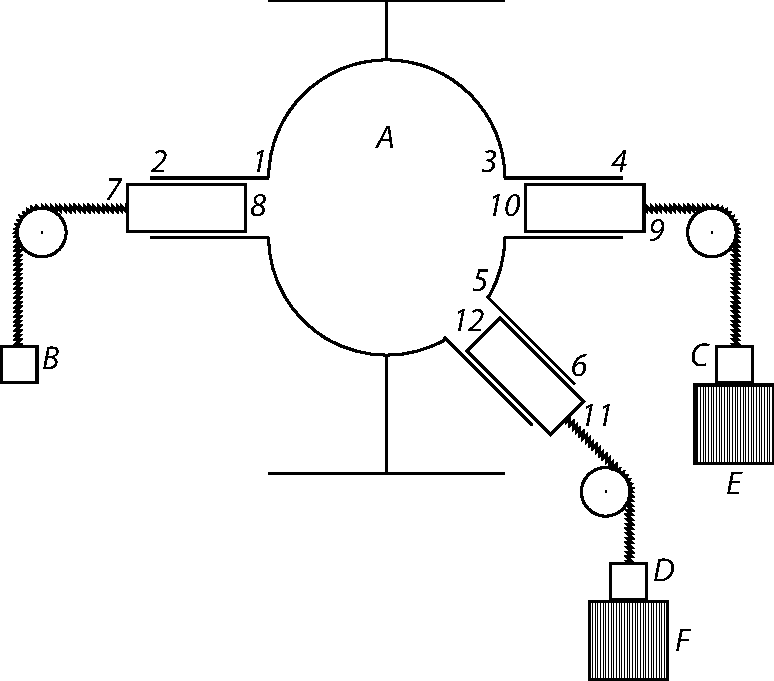
\includegraphics[width=0.62\textwidth]{gesamttex/edit_VIII,3/images/LH_35_10_17_005-008_d2.pdf}}%
%  \vspace*{0.5em}
%  \centerline{\lbrack\textit{Fig.~2; L\textsuperscript{1}\! (Bl.~7~v\textsuperscript{o}\!; 8~r\textsuperscript{o}\!) u. L\textsuperscript{2}\! (Bl.~6~r\textsuperscript{o}\!)}\rbrack}\label{LH_35_10_17_008r_Fig2}%
%%
%  \newpage
%  \vspace*{2.0em}%
%
%
\pstart%
Caeterum supposuimus hactenus
tubos\protect\index{Sachverzeichnis}{tubus} esse
diametris\protect\index{Sachverzeichnis}{diameter tubi} aequales,
sed si inaequales \makebox[1.0\textwidth][s]{sint,
etiam pondera non erunt aequalia,
sed capacitatibus tuborum\protect\index{Sachverzeichnis}{capacitas tubi}
(\protect\vphantom)%
id est quadratis ab}
\pend
\newpage
  \centerline{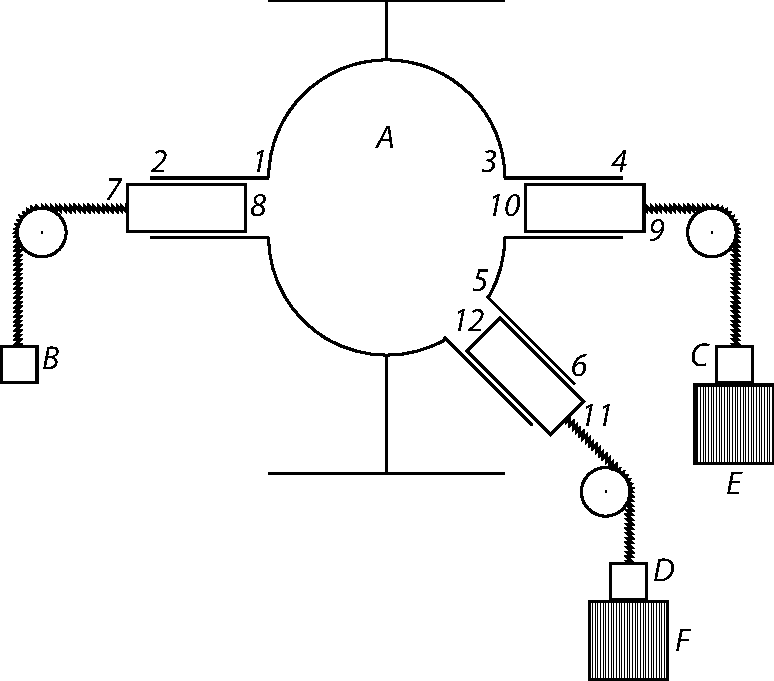
\includegraphics[width=0.64\textwidth]{gesamttex/edit_VIII,3/images/LH_35_10_17_005-008_d2.pdf}}%
  \vspace{0.5em}
  \centerline{\lbrack\textit{Fig.~2; L\textsuperscript{1}\! (Bl.~7~v\textsuperscript{o}\!; 8~r\textsuperscript{o}\!) u. L\textsuperscript{2}\! (Bl.~6~r\textsuperscript{o}\!)}\rbrack}\label{LH_35_10_17_008r_Fig2}%
  \vspace{2.0em}
\pstart\noindent%
\edtext{}{\lemma{\hspace{1,6mm}\lbrack\textit{Fig.~2}\rbrack}\killnumber\Cfootnote{%
In \textit{L\textsuperscript{1}} zweifach ausgeführt. % (Bl.~7~v\textsuperscript{o}\! und Bl.~8~r\textsuperscript{o}\!).
In der Fassung auf Bl.~8~r\textsuperscript{o} heißt die Stütze \textit{E} irrtümlich \textit{Q}.}}%
eorum diametris\protect\index{Sachverzeichnis}{diameter tubi}%
\protect\vphantom()
reciproce proportionalia.
Hanc enim in rem sufficit considerari pondera duo \textit{B} et \textit{C}, cum suis tubis%
\edlabel{LH_35_10_17_007r-007v_strch-2}
%%%%%
\edtext{\textit{1.2} et \lbrack\textit{3.4},\rbrack}{%
\lemma{\textit{1.2}}\Bfootnote{\hspace{-0,5mm}% 
et \textit{2.3},%
~\textit{L\textsuperscript{1}}
\hspace{0,5mm}\textit{1.2} et
\textbar~\textit{2.3}, \textit{ändert Hrsg.}~\textbar%
~\textit{L\textsuperscript{2}}}}
%
ubi si tubi\protect\index{Sachverzeichnis}{tubus} sint
%
\edtext{inaequales diametris,\protect\index{Sachverzeichnis}{diameter tubi}
et \textit{1.2} major, ac \textit{3.4} minor\lbrack,\rbrack}{%
\lemma{inaequales}\Bfootnote{\hspace{-0,5mm}%
\textbar~diametris \textit{erg.}~%
\textbar\ et \textit{1.2} major at \textit{3.4} minor%
~\textit{L\textsuperscript{1}}\hspace{0,5mm}
inaequales diametris, \lbrack...\rbrack\ \textit{3.4} minor%
~\textit{L\textsuperscript{2}}}}
%
tunc descendente pondere\protect\index{Sachverzeichnis}{pondus descendens}
\edtext{\textit{B}}{%
\lemma{\textit{B}~,~\textit{L\textsuperscript{1}}}\Bfootnote{%
\hspace{0,5mm}%
\textit{B}~\textit{L\textsuperscript{2}}}}
%
et attrahente pondus\protect\index{Sachverzeichnis}{pondus attractum}
%
\edtext{\textit{C}}{%
\lemma{\textit{C}~,~\textit{L\textsuperscript{1}}}\Bfootnote{%
\hspace{0,5mm}%
\textit{C}~\textit{L\textsuperscript{2}}}}
%
sine fluidi dilatatione\protect\index{Sachverzeichnis}{dilatatio fluidi}
per solum ejus motum\protect\index{Sachverzeichnis}{motus fluidi}
%
\edtext{(\protect\vphantom)%
ut si fluidum\protect\index{Sachverzeichnis}{fluidum tendibile}
esset non aer\protect\index{Sachverzeichnis}{aer} sed aqua,\protect\index{Sachverzeichnis}{aqua}
fingendo attractionem,\protect\index{Sachverzeichnis}{attractio ponderis}
etsi ea revera a circumpulsione\protect\index{Sachverzeichnis}{circumpulsio} oriatur\protect\vphantom()}{%
\lemma{\hspace{-0,5mm}(\protect\vphantom)ut}\Bfootnote{%
\hspace{-0,5mm}si \lbrack...\rbrack\ sed aqua\protect\vphantom()
\textit{erg.~L\textsuperscript{1}}
\hspace{0,5mm}(\protect\vphantom)ut si \lbrack...\rbrack\ circumpulsione oriatur\protect\vphantom()%
~\textit{L\textsuperscript{2}}}}
%
pondus \textit{C} ascendit
\edtext{tanto magis}{%
\lemma{tanto}\Bfootnote{%
\textit{(1)}~minus
\textit{(2)}~magis%
~\textit{L\textsuperscript{1}}}}
%
quam \textit{B} descenderat,
quanto tubus \textit{3.4} est minus capax tubo \textit{1.2}.\protect\index{Sachverzeichnis}{tubus}
Itaque aequilibrium\protect\index{Sachverzeichnis}{aequilibrium}
\edtext{erit}{%
\lemma{erit~,~\textit{L\textsuperscript{1}}}\Bfootnote{%
\hspace{0,5mm}erit%
~\textit{L\textsuperscript{2}}}}
%
si pondera\protect\index{Sachverzeichnis}{pondus ascendens}\protect\index{Sachverzeichnis}{pondus descendens}
sint reciproce ut capacitates tuborum.\protect\index{Sachverzeichnis}{capacitas tubi}
Unde cognoscimus tensiones\protect\index{Sachverzeichnis}{tensio fluidi} non
\edtext{tantum ponderibus\protect\index{Sachverzeichnis}{pondus tendens}}{%
\lemma{tantum}\Bfootnote{\hspace{-0,5mm}%
ponderibus,%
~\textit{L\textsuperscript{1}}
\hspace{0,5mm}tantum
\textit{(1)}~ponderibus,
\textit{(2)}~ponderibus%
~\textit{L\textsuperscript{2}}}}
%
sed et ponderum in rem tendibilem\protect\index{Sachverzeichnis}{res tendibilis}
effectibus\protect\index{Sachverzeichnis}{effectus ponderis} esse
\edlabel{LH_35_10_17_006v_strch-1}aestimandas.\protect\index{Sachverzeichnis}{aestimatio tensionis}
\edtext{}{%
{\xxref{LH_35_10_17_006v_strch-1}{LH_35_10_17_006v_strch-2}}
{\lemma{aestimandas}\Bfootnote{%
\textit{(1)}~, et duos tubos inaequales quodammodo repraesentare
\textit{(a)}~duo
\textit{(b)}~unam chordam inae
\textit{(c)}~duas extremitates ejusdem chordae
\textit{(aa)}~in
\textit{(bb)}~crassitie inaequales
\textit{(2)}~. Sed quod \lbrack...\rbrack\ tubis inaequalibus % de duobus
\textbar~ejusdem vasis \textit{erg.}~%
\textbar\ diximus, non
\textit{(a)}~debet
\textit{(b)}~potest applicari \lbrack...\rbrack\ crassitiei habentem.%
~\textit{L\textsuperscript{1}}}}}
\pend%
%
%
\pstart%
Sed quod de duobus tubis\protect\index{Sachverzeichnis}{tubus}
inaequalibus ejusdem vasis\protect\index{Sachverzeichnis}{vas}
diximus, %\edtext{}{%\lemma{diximus}\Cfootnote{%??? Überflussig, weil unmittelbar davor.}}
non potest applicari ad chordam
duas extremitates\protect\index{Sachverzeichnis}{extremitas chordae}
inaequalis crassitiei\protect\index{Sachverzeichnis}{crassities chordae} habentem.%
\edlabel{LH_35_10_17_006v_strch-2}
%%
Nam utcunque se habeat chorda,\protect\index{Sachverzeichnis}{chorda tensa}
non
\edtext{potest moveri}{%
\lemma{potest}\Bfootnote{%
\hspace{-0,5mm}\textbar~chorda \textit{gestr.}~\textbar\ moveri%
~\textit{L\textsuperscript{1}}}}
sine tensione,\protect\index{Sachverzeichnis}{tensio chordae}
quin unum pondus tantum ascendat,\protect\index{Sachverzeichnis}{pondus ascendens}
%
\edtext{quantum descendit alterum;\protect\index{Sachverzeichnis}{pondus descendens}
quod secus erat in tubis inaequalibus,
ubi pondus tubi amplioris embolum\protect\index{Sachverzeichnis}{embolus tractus}
trahens\protect\index{Sachverzeichnis}{pondus trahens} minus descendit,
quam alterum ascendere necesse est.
Interim verum}{%
\lemma{quantum}\Bfootnote{\hspace{-0,5mm}%
\textbar~descendit \textit{erg.}~%
\textbar\ alterum. Interim verum%
~\textit{L\textsuperscript{1}}\hspace{0,5mm}
quantum descendit alterum
\textit{(1)}~. Interim verum
\textit{(2)}~; quod secus
\textit{(a)}~erit 
\textit{(b)}~erat in \lbrack...\rbrack\ ubi pondus % tubis inaequalibus,
\textit{(aa)}~ad totum
\textit{(bb)}~tubi amplioris \lbrack...\rbrack\ Interim verum%
~\textit{L\textsuperscript{2}}}}
%
est chordam\protect\index{Sachverzeichnis}{chorda tensa}
pluribus filis\protect\index{Sachverzeichnis}{filum}
constantem\protect\index{Sachverzeichnis}{chorda pluribus filis constans}
ab eodem pondere minus tendi,\protect\index{Sachverzeichnis}{pondus tendens}
et duplicata chorda\protect\index{Sachverzeichnis}{chorda duplicata}
fore dimidiam
%
\edtext{in singulis}{%
\lemma{in}\Bfootnote{%
partibus~\textit{L\textsuperscript{1}}\hspace{0,5mm}
in singulis~\textit{L\textsuperscript{2}}}}
%
tensionem.\protect\index{Sachverzeichnis}{tensio chordae}
%
Itaque verum est hic quoque
\edtext{pondera,\protect\index{Sachverzeichnis}{pondus tendens}
sed aeque ambo, minus descendere}{%
\lemma{pondera,}\Bfootnote{%
\textit{(1)}~sed ambo simul, minus descendere
\textit{(2)}~sed aeque ambo, minus descendere%
~\textit{L\textsuperscript{1}}}}
%
ad eandem vim\protect\index{Sachverzeichnis}{vis tonica}
%
\edtext{tonicam in chorda multiplicata,\protect\index{Sachverzeichnis}{chorda multiplicata}
efficiendam. Et}{%
\lemma{tonicam}\Bfootnote{\hspace{-0,5mm}%
\textit{(1)}~chordae
\textit{(2)}~in chorda
\textit{(a)}~crassiori
\textit{(b)}~multiplicata
\textit{(aa)}~efficienda,
\textit{(bb)}~efficiendam,
\textit{(aaa)}~adeoque
\textit{(bbb)}~et%
~\textit{L\textsuperscript{1}}\hspace{0,5mm}
tonicam in \lbrack...\rbrack\ efficiendam. Et% chorda multiplicata,
~\textit{L\textsuperscript{2}}}}
%
tensiones\protect\index{Sachverzeichnis}{tensio chordae}
in eadem chorda\protect\index{Sachverzeichnis}{chorda tensa}
%
\edtext{diversae multiplicitatis\protect\index{Sachverzeichnis}{multiplicitas chordae}
seu crassitiei\protect\index{Sachverzeichnis}{crassities chordae}}{%
\lemma{diversae}\Bfootnote{\hspace{-0,5mm}%
\textit{(1)}~crassitiei
\textit{(2)}~crassitudinis,
\textit{(3)}~multiplicitatis,%
~\textit{L\textsuperscript{1}}\hspace{0,5mm}
diversae multiplicitatis seu crassitiei%
~\textit{L\textsuperscript{2}}}}
%
esse crassitiebus\protect\index{Sachverzeichnis}{crassities filorum}
\edtext{seu numeris filorum\protect\index{Sachverzeichnis}{numerus filorum}}{%
\lemma{seu}\Bfootnote{%
\hspace{-0,5mm}numeris filorum
\textit{erg.~L\textsuperscript{1}}}}
%
reciproce
\edtext{proportionales,}{%
\lemma{proportionales~;~\textit{L\textsuperscript{1}}}\Bfootnote{%
\hspace{0,5mm}
proportionales~,~\textit{L\textsuperscript{2}}}}
%
vi\protect\index{Sachverzeichnis}{vis tonica}
\edtext{tonica
(\protect\vphantom)%
quae in ratione est composita numeri repetitionum,\protect\index{Sachverzeichnis}{repetitio}
et tensionis\protect\index{Sachverzeichnis}{tensio chordae}
in quavis chorda simplice%
\protect\vphantom()
semper}{%
\lemma{tonica}\Bfootnote{\hspace{-0,5mm}%
\textbar~in chordae partibus \textit{erg.}~%
\textbar\ ubique%
~\textit{L\textsuperscript{1}}
\hspace{0,5mm}tonica
\textit{(1)}~licet
\textit{(2)}~(\protect\vphantom)quae in ratione est composita
\textit{(a)}~filorum
\textit{(b)}~numeri repetitionum, \lbrack...\rbrack\ chorda simplice\protect\vphantom()
\textit{(aa)}~ubique
\textit{(bb)}~semper%
~\textit{L\textsuperscript{2}}}}
aequali existente,
%
et\protect\index{Sachverzeichnis}{pondus tendens}
\edtext{per alterutrum ponderum
(\protect\vphantom)%
utique aequalium%
\protect\vphantom()}{%
\lemma{per}\Bfootnote{\hspace{-0,5mm}%
\textit{(1)}~pondus
\textit{(2)}~alterutrum ponderum, utique aequalium,%
~\textit{L\textsuperscript{1}}\hspace{0,5mm}
per alterutrum ponderum (\protect\vphantom)utique aequalium\protect\vphantom()%
~\textit{L\textsuperscript{2}}}}
aestimanda.%
% % % % %    ACHTUNG GETRIXT: FOLGENDE CFOOTNOTE HÄNGT AN FIG. 3    ! ! ! ! 
% \edtext{}{\lemma{\hspace{1,6mm}\lbrack\textit{Fig.~3}\rbrack}\killnumber\Cfootnote{%
% In \textit{L\textsuperscript{1}} auf Bl.~8~v.}}
% % % % %    ACHTUNG GETRIXT: FOLGENDE CFOOTNOTE HÄNGT AN FIG. 2    ! ! ! ! 
\pend%
%  \vspace*{2.0em}%
%
%
%  \newpage
  \vspace{2.0em}%
%
  \centerline{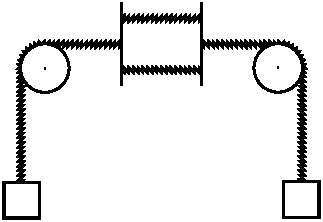
\includegraphics[width=0.30\textwidth]{gesamttex/edit_VIII,3/images/LH_35_10_17_005-008_d3.pdf}}%
  \vspace*{1.0em}
  \centerline{\lbrack\textit{Fig.~3; L\textsuperscript{1} (Bl.~8~v\textsuperscript{o}\!) u. L\textsuperscript{2} (Bl.~6~r\textsuperscript{o}\!)}\rbrack}%
  \count\Bfootins=1200
\count\Afootins=1200
\count\Cfootins=1200
%
%  \vspace*{2.0em}%
%
% ENDE DES STÜCKES auf Blatt 6r (L2) bzw 8v (L1).